\chapter{Algorithmen zur Pfadplanung}
\section{Was sind Algorithmen zur Pfadplanung?}
%Es stellt sich die Frage was ein Pfadplanungsalgorithmus "uberhaupt ist, nach [Lavalle] ist es nicht sinnvoll eine genaue Mathematische Definition abzugeben, sondern das Ziel ist eine generelle Idee zu vermitteln und diese mit Beispielen zu veranschaulichen.
%Als eine Antwort zu der Frage wird eine Turing Maschine beschrieben, da damit die meisten Pfadplanungsalgorithmen modelliert werden k"onnen. Turing Maschinen sind "finite-state-machines" welche informationen als String einlesen, diese verarbeiten und aktzeptieren oder ablehnen k"onnen. 
%Mit einer Erweiterung dieses Konzepts kann am Ende auch ein Pfadplan ausgegeben werden. Das Problem bei der Pfadplanung kommt daher, dass die Maschine auf die Umgebung oft reagieren muss, und informationen die durch Sensoren gegeben werden mit einbeziehen m"ussen. 
%Dadurch gibt es keine klare Trennung von der Umwelt und der Maschine solange nicht alle Daten dem System im Vorhinein bekannt sind.[Lavalle]
%\newline
%Ein Ansatzpunkt w"are ein \"on-line algorithmus" der sich aktiv aktualisiert, aber auch dieser kann nicht die gesamte komplexit"at wiederspiegeln. 

Algorithmen zur Pfadplanung sind schwierig mathematisch pr"azise zu definieren. Ein Ansatz ist eine Definition für einen Algorithmus abzugeben und diese anschlie"send zu erweitern, sodass sie den Anspr"uchen der Pfadplanung entspricht. Nach der Church-Turing These ist ein Algorithmus eine Turing Maschine cite{462,891}. Dieser Definition fehlt aber unter anderem, die Repr"asentation der Interaktion eines Roboters mit der Umgebung, wie es in \ref{lav01} dargestellt wird. Daher wird ein Planer \footnote{Planer (engl. planner)} als ein Algorithmus definiert, welcher einen Plan \footnote{Plan (engl. plan)} konstruiert. Der Planer kann sowohl eine Maschine als auch ein Mensch sein und kann dem Konzept einer Turing Maschine entsprechen. Er ist aber nicht darauf limitiert, sondern kann den Anspr"uchen entsprechend erweitert werden.\cite[~S. 19ff]{Lav06} 

\begin{figure} % Hier lieber eine eigene Kombination an Grafiken
	\centering
	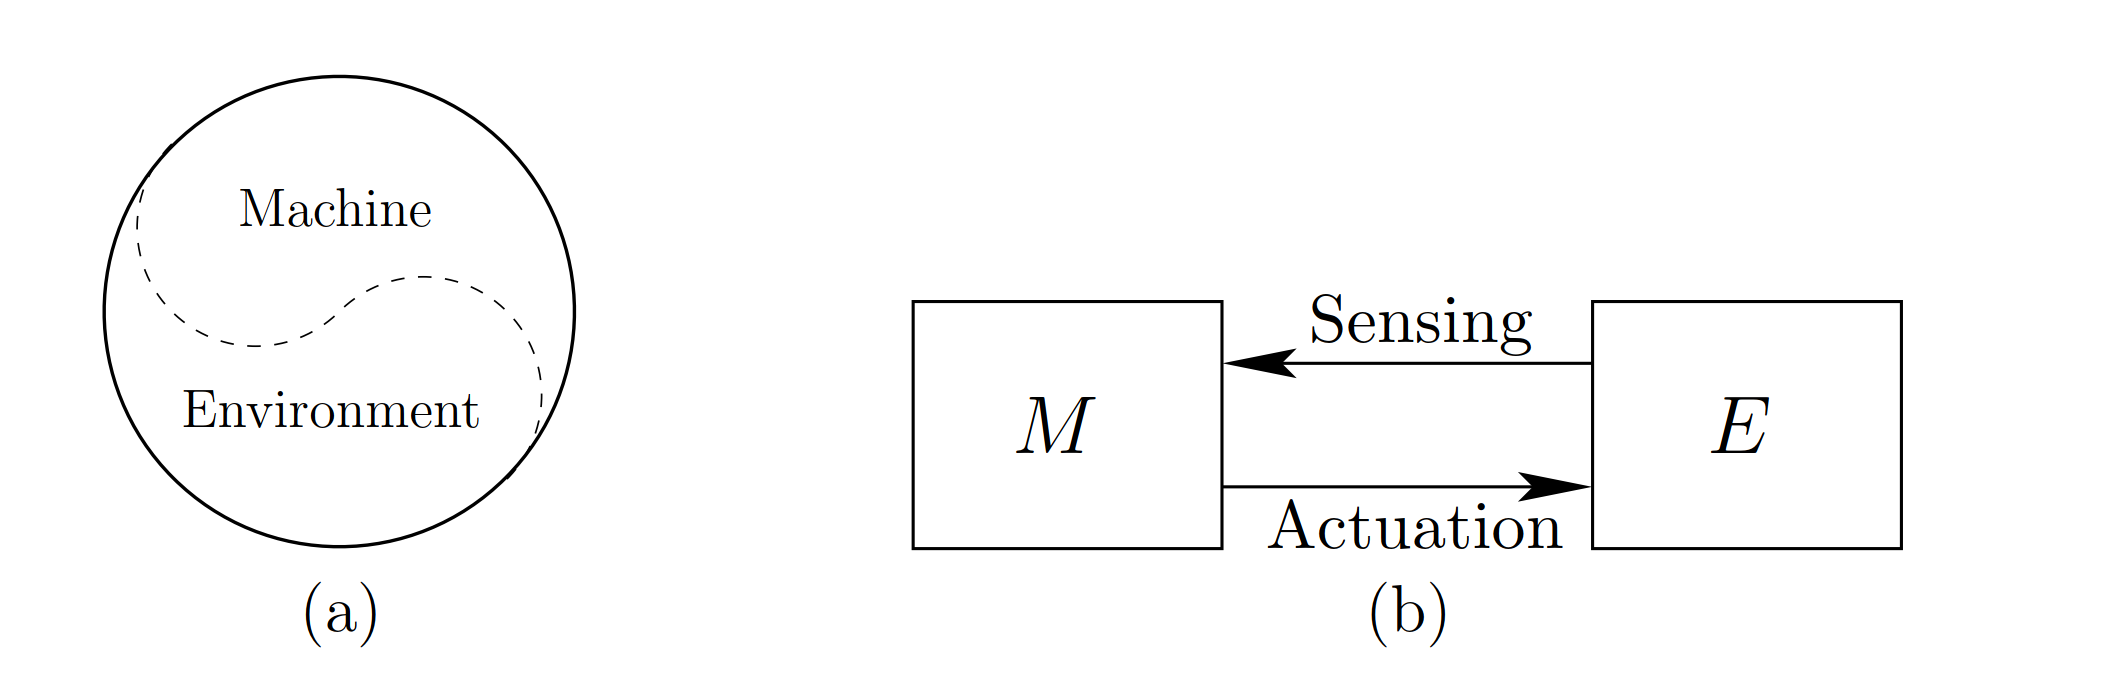
\includegraphics[width=0.6\textwidth]{images/img224.png}
	\caption{Abb. 1.5 von \cite[~S. 20]{Lav06}:  (a) Die Grenze zwischen Maschine und Umgebung ist flie"send, es ist eine Linie die stark in Abh"angigkeit vom Kontext gezogen wird. (b) Ist die Grenze festgelegt, wird angenommen, dass die Maschine M mit der Umgebung U durch Sensorik und den Antrieb interagiert.}
	\label{lav01}
\end{figure}
 



Ein solcher Plan, kann drei unterschiedliche Funktionen erf"ullen. Darunter fallen die Ausf"uhrung \footnote{Ausf"uhrung (engl. Execution)} der Anweisungen in einer Simulation oder durch einen Roboter, die Verbesserung\footnote{Verbesserung (engl. Refinement)} der Eigenschaften in bestimmten Parametern und die hierarchische Einbindung \footnote{Hierarchische Einbindung (engl. Hierarchical Inclusion)} des Plans.
%Ausführung
Pl"ane k"onnen auf zwei weisen ausgef"uhrt werden. Zum einen kann ein Plan als kodierte Eingabe f"ur eine Maschine erstellt werden, welche dadurch programmiert werden kann. Auf diese weise wird die Maschine bei der Ausf"uhrung autonom und kann nicht mehr mit dem Planer interagieren. 
Im zweiten Fall erzeugt der Planer eine Spezialmaschine \footnote{Spezialmaschine (engl. special-purpose machine)}, welche dazu entworfen ist eine Aufgabe zu l"osen.
\newline\\
%Verbesserung
Um einen Plan zu verbessern, wird dieser als Eingabe einem Planer "ubergeben, der daraus einen verbesserten Plan erzeugen soll. 
Anhand von \ref{lav02} wird ersichtlich, wie der gleiche Plan verbessert werden kann, indem verschiedene Aspekte der Problemstellung fokussiert werden.
Die Auswahl der richtigen Kriterien ist schon seit l"angerer Zeit ein Forschungsgebiet in der Robotik, da auch hier Vor- und Nachteile mit verschiedenen Kriterien einhergehen.
\newline\\
%Hierarchische Einbindung
Bei der Hierarchischen Einbindung, wird ein Baum aus Pl"anen erzeugt. Dabei steht an der Wurzel der Hauptplan \footnote{Hauptplan (engl. masterplan)}, welcher andere Pl"ane als Bl"atter in einer Hierarchie einbindet. Ein Plan wird als Aktion betrachtet, die nur als Teil des Gesamtsystem funktioniert. Es wird dadurch erreicht, dass die Abgrenzung zwischen Maschine und Umgebung an verschiedenen stellen gezogen wird.
\newline\cite[~S. 21ff]{Lav06} 

\begin{figure} % Hier lieber eine eigene Kombination an Grafiken
	\centering
	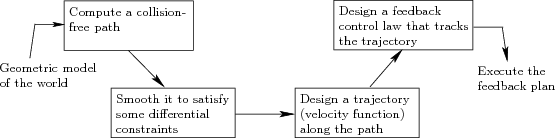
\includegraphics[width=0.6\textwidth]{images/img247.png}
	\caption{Abb. 1.5 von \cite[~S. 20]{Lav06}:  Ein Verbesserungsprozess, der sich in der Robotik bew"ahrt hat.}
	\label{lav02}
\end{figure}

\section{Klassifizierung von Pfadplanungsalgorithmen} % Hier bitte noch ein Bild, das die Unterschiede der einzelnen Klassen sichtbar macht. 
Der Bereich der Pfadplanung ist "au"serst heterogen, da die Umsetzung der Pfadplanung stark von den Vorgaben des Einsatzgebiets abh"angt. 
Es wird Planen in einem diskreten und in einem kontinuierlichen Zustandsraum\footnote{Zustandsraum (engl. state space) Der Zustandsraum beschreibt alle potentiell aufkommenden Zust"ande.} unterschieden. Planen in einem kontinuierlichen Zustandsraum wird Bewegungsplanung genannt, dabei klassifiziert man zwischen Planung mit allen Umgebungsinformationen vorhanden, Planen mit Unsicherheit, sowie Planung mit Bewegungseinschr"ankungen.
Auf die genaue Einteilung der Einsatzgebiete wird in \ref{Kapitel5} noch eingegangen, jedoch ist es f"ur das Verst"andnis der Algorithmen wichtig eine Einsch"atzung der verschiedenen Anforderungen zu erhalten. Im folgenden behandeln wir vor allem die diskrete Pfadplanung, da man daran die Grundlagen erkl"aren kann. \cite[~S. 24ff]{Lav06} 

\section{Diskrete Pfadplanung} \label{Kapitel 4.3} % In diesem Kapitel hätte ich gerne noch ein Bild, das das Konzept der diskreten Pfadplanung auf einen Blick veranschaulicht veranschaulicht

Diskrete Pfadplanung dient in der meisten Literatur als Einstiegspunkt. Das kommt daher, da der state space entweder endlich oder z"ahlbar unendlich ist.\\
Au"serdem müssen dadurch keine geometrischen Modelle oder Bewegungseinschr"ankungen \footnote{Bewegungseinschr"ankungen (engl. differential constraints)} im Entwurf des Algorithmus beachtet werden.
% Der Planer weis über alles bescheit, die struktur ist regelmaeßig
Je nach Anforderung werden die drei Teilgebiete feasible planning \footnote{feasible planning (Dt. durchführbares Planen) im folgenden FP}, optimales planen und logik basierte repr"asentation unterschieden. Die vorherrschenden Algorithmen in diesem Bereich, sind der Dijkstra Algorithmus aus der Graphentheorie und der daraus abgeleitete A*-Algorithmus. Von diesem gibt es noch eine Reihe weiterer Abwandlungen, die alle eine Optimierung auf ein bestimmtes Einsatzgebiet zum Ziel haben.\cite[~S. 27]{Lav06} \\
Wie man diese Optimierung durchführen kann wird im folgenden an verschiedenen Algorithmen erl"autert. Optimales Planen unterscheidet sich nur insofern vom feasible planning, als das der gefundene Pfad in verschiedenen Kriterien wie Zeit, Distanz oder auch der Anzahl an Drehungen eines Roboters optimiert werden kann.\cite[~S. 43]{Lav06} \\
Der state space spielt in der Pfadplanung eine zentrale Rolle, dabei kann zwischen Zust"anden durch die Ausf"uhrung von Aktionen gewechselt werden. Die verf"ugbaren Aktionen werden in einem Aktiosraum\footnote{Aktionsraum (engl. action space) } zusammengefasst, au"serdem ist als Teil des Planungsproblem ein Satz von Zielzust"anden\footnote{Zielzust"ande (engl. goal states)} definiert. 
Da ein Zustandsgraph schnell sehr gro"s werden kann wird dieser meist nicht komplett "ubergebe, sondern diese wird im Laufe des Planungsprozess aufgedeckt.
\cite[~S. 43]{Lav06} \\
Wie man effektiv durch den Zustandsraum navigiert um einen goal state zu erreichen ist das Thema des folgenden Absatz.
\begin{figure}
\centering
\subsection*{Formulierung 4.3 (Discrete Feasible Planning)}
\begin{enumerate}
	\item Ein nichtleerer Zustandsraum $X$, der endlich viele oder z"ahlbar unendlich viele Zust"ande beschreibt.  
	\item F"ur jeden Zustand $x \in X$ , ein endlicher Aktionsraum $U( \, x) \,$.
	\item Eine Zustands"ubergangsfunktion $f$ welche einen Zustand  $f( \, x,u) \, \in X$ für jedes $x \in X$  und $u \in U( \, x) \,$ erzeugt. Die Zustands"ubergangsgleichung ist von $f$ als $x' = f( \, x,u )\, $ abgeleitet.
	\item Ein Anfangszustand $ x_{I} \in X$.
	\item Ein Satz mit Zielzust"anden $X_{G} \subset X$.
\end{enumerate}
\caption{In Anlehnung an Formulation 2.1 von \cite[~S. 29]{Lav06}}
\label{lav02}
\end{figure}
%1. A nonempty state space X, which is a finite or countably infinite set of states.
%2. For each state x ∈ X, a finite action space U(x).
%3. A state transition function f that produces a state f(x, u) ∈ X for every
%x ∈ X and u ∈ U(x). The state transition equation is derived from f as
%x′ = f(x, u).
%4. An initial state xI ∈ X.
%5. A goal set XG ⊂ X.

\subsection {Feasible Planning} % Hier sollte mit einem Code Beispiel ein allgemeingültiger algorithmus veranschaulicht werden. Darauf kann dann später wieder eingegangen werden und veränderungen im code können mit veränderungen in der Funktionalität in kontakt gesetzt werden.
Ein allgemeiner Beispielalgorithmus ist in [Lavalle] gegeben. Als Beispiel f"ur diskrete Pfadplanung kann die Bewegung auf einem endlichen 2D Netz mit Hindernissen gesehen werden. 
Dieses hat einen Startpunkt und einen Zielpunkt und muss einen Pfad zwischen diesen Punkten finden. Bei der Feasible Planning ist es ausreichend einen funktionierenden Pfad zu finden und es wird noch nicht darauf geachtet ob dieser optimal in Hinblick auf L"ange ist.
\newline
Die Algorithmen die hier verwendet werden sind Algorithmen zur Graphensuche die das Problem aus einer Planungsperspektive angehen. Es ist wichtig, dass diese Algorithmen systematisch sind. Das bedeutet, dass bei einem endlichen Graphen alle zust"ande besucht werden, au"serdem muss beachtet werden welche Zust"ande schon besucht wurden. Bei einem unendlichen Graphen ist die Definition insofern anders ist, dass es ausreicht, dass der Algorithmus zu einer L"osung bei l"osbaren Problemen kommt. 
\newline 
Eine generelle Template f"ur einen Suchalgorithmus kann durch drei Zust"ande repr"asentiert werden. 
Ein unentdecktes Feld wurde noch nicht besucht und ist daher auch noch nicht bekannt. Ein Totes Feld kann nichts mehr zur Suche Beitragen, da schon die angrenzenden Felder entdeckt wurden. Felder die noch am Leben sind haben noch potentielle Nachbarfelder die am leben sind.  
\newline
Der einzige wirkliche Unterschied zwischen Planungsalgorithmen kommt durch die Auswahl eines Sortieralgorithmus f"ur die Priority Queue in welcher die n"achsten abzuarbeitenden Elemente enthalten sind. Die einfachsten Varianten sind hier FIFO(First-In First-Out), hier wird immer das Element gew"ahlt das am l"angsten gewartet hat. Dadurch entsteht eine kreisf"ormig expandierende Suche. 
\newline
Damit der gefundene Weg vom Start zum Ziel rekonstruiert werden kann muss jeder Knoten seinen Vorg"angerknoten abspeichern. Das erm"oglicht es den Weg sp"ater zur"uckzuverfolgen. 
\newline
Um darzustellen welchen einfluss die Sortierfunktion auf das Verhalten der Algorithmus hat werden im folgenden einige Algorithmen pr"asentiert.
Diese sind alle eine Abwandlung des Algorithmus aus der Abbildung. 
\newline
\newline
\subsubsection{Breath-first search} Breadth first search verwendet die oben angesprochene FIFO Warteschlange wodurch sich eine kreisf"ormige expansion ergibt, die auch die vorraussetzung f"ur systematische Algorithmen erf"ullt. Bei diesem algorithmus k"onnen einige kontrollmechanismen eingespart werden die sonst zur kontrolle der Expanionn"otig werden, jedoch verschwendet dieser Algorithmus durch die gleichm"assige ausbreitung relativ viele Zyklen. 
\newline
\newline
\subsubsection{Depth first search} Depth first search verwendet einen Stack als warteschlange, das heisst LIFO(Last-In First-Out) dies erzeugt eine aggresive Expansion in eine bestimmte Richtung.
Da die Richtung in die am anfang zum expandieren gew"ahlt wird zuf"allig ist, ist diese Methode nicht wirklich zielf"uhrend, da sie nur bei endlich vielen Knoten systematisch ist. 
\subsubsection{Djikstra Algorithmus}
Der Djiksta Algorithmus findet einen optimalen Pfad kann aber auch feasible pfade finden. Der Unterschied zu den vorhergehenden Algorithmen ist das hier Aktionen mit einander verglichen werden um die die mit den besseren Chancen ein gutes ergebnis zu finden erst auszuf"uhren. Das vorgehen von Dijkstra ist weitgehend bekannt und kann bei [Lavalle] nachgelesen werden.

\subsubsection{A-Stern} 
Der A* Suchalgorithmus ist eine Erweiterung von Dijkstra's Algorithmus und mit dem Ziel, die Anzahl der gesamtschritte zu minimieren,
indem eine Heuristik eingef"uhrt wird die die Suche in die Richtung des Ziels f"uhrt. Dabei k"onnen unterschiedliche Werte f"ur die Heuristik gew"ahlt werden,
jedoch wird meistens die der direkte Abstand zwischen dem Start und dem Endpunkt als Wert genommen. Das daraus entstehende verhalten zeichnet sich dadurch aus dass der Algorithmus solange in die Richtun des Ziels sucht, bis er auf ein hindernis st"o"st und erst dann versucht dieses Hindernis zu umgehen.
\newline
TODO Mehr informationen
\subsubsection{weitere}
Weitere Abwandlungen sind Best first search, hier wird die Warteschlange nach einer erwarteten \"cost-to-go" sortiert. 
Desweiteren gibt es noch abwandlungen wie Interative Deepening das den Depth first Algorithmus in abgewandelter form einsetzt. 
R"uckw"artssuche und Bidirektionale suche verhalten sich so wie ihr es beschreibt und kommen alle mit eigenheiten. 


%Simon fährt fort
\section{Planung mit kontinuierlichem Zustandsraum}
Lorem ipsum dolor sit amet, consetetur sadipscing elitr, sed diam nonumy eirmod tempor invidunt ut labore et dolore magna aliquyam erat, sed diam voluptua. At vero eos et accusam et justo duo dolores et ea rebum. Stet clita kasd gubergren, no sea takimata sanctus est Lorem ipsum dolor sit amet. Lorem ipsum dolor sit amet, consetetur sadipscing elitr, sed diam nonumy eirmod tempor invidunt ut labore et dolore magna aliquyam erat, sed diam voluptua. At vero eos et accusam et justo duo dolores et ea rebum. Stet clita kasd gubergren, no sea takimata sanctus est Lorem ipsum dolor sit amet.

 
%%oder einer Grafik die ich noch schreiben muss. 
%\section{Bewegungsplanung}
%% Die Planung muss zus"atzlich noch die Bewegung in der Umgebung in betracht ziehen. 
%\subsection{Sampling-Based Motion Planning}
%\subsection{Combinatorial Motion Planning}
%\section{Planen mit Unsicherheit}
%% Hier kommt noch unsicherheit in der Umgebung hinzu, also auch dynamische Systeme
%\subsection{Entscheidungstheorie}
%\subsection{Planen mit Unsicherheiten in der Sensorik}
%\section{Planen mit Differentialen Einschr"ankungen}
%% Hier müssen bewegungseinschr"ankungen die durch den Verwendeten Roboter einhergehen beachtet werden. 
%\subsection{Sampling-Based Planning under Differential Constraints}
